\section{Υλοποίηση}

\paragraph{} Η προσομοίωση αποτελείται από δύο βασικά στοιχεία, την ακτογραμμή
(\eng{terrain}) και το ρευστό (\eng{fluid}). Το ρευστό είναι το δυναμικό στοιχείο, σε
αντίθεση με τη στατική ακτογραμμή. Στο πρόγραμμα προσομοίωσης, που στηρίζεται στη μηχανή
φυσικής \eng{Bullet}, δίνονται οι αρχικές συνθήκες του ρευστού (θέση και ταχύτητα) και
εισάγεται η ακτογραμμή με τη μορφή τρισδιάστατου τριγωνικού δικτύου επιφάνειας
(\eng{triangle surface mesh}). Στη συνέχεια εκτελείται η προσομοίωση και τα δεδομένα
εξάγονται σε αρχεία τύπου \eng{VTK} που μπορούν εισαχθούν σε ένα από τα πολλά προγράμματα
οπτικοποίησης που είναι διαθέσιμα ελεύθερα (λ.χ. \eng{ParaView}).

\subsection{Γενική αρχιτεκτονική}
\paragraph{} Το πρόγραμμα προσομοίωσης στηρίζεται στην αλληλεπίδραση της \eng{Bullet} και
της μηχανής \eng{SPH} που αναπτύχθηκε ενώ στην εικόνα \ref{fig:architecture}
απεικονίζονται διαγραμματικά οι αλληλεξαρτήσεις μεταξύ των κυριότερων τμημάτων της
εφαρμογής και η ροή της πληροφορίας εισόδου και εξόδου. Τα δεδομένα εισόδου αποτελούνται
από το τρισδιάστατο μοντέλο της ακτογραμμής και οι αρχικές συνθήκες του ρευστού, ενώ η
εξαγόμενη πληροφορία αφορά τις ώσεις που δέχθηκε η ακτογραμμή, αλλά και πληροφορίες
σχετικά το ίδιο το ρευστό και δεδομένα που σχετίζονται με τη ροή.

\paragraph{} Η είσοδος της προσομοίωσης αντιπροσωπεύει τις αρχικές συνθήκες του ρευστού
και το μοντέλο της ακτογραμμής. Όπως θα εξηγηθεί και στα αποτελέσματα, λόγω της φύσης των
τσουνάμι, επελέγη μοντελοποίηση αυτών με ενιαίο όγκο νερού που κατευθύνεται προς την
ακτογραμμή με σταθερή ταχύτητα. Λόγω αυτού, κατά την είσαγωγή των δεδομένων είναι αναγκαίο
να προσδιοριστεί η αρχική θέση και ταχύτητα του ρευστού, αλλά και το επιθυμητό επίπεδο
ανάλυσης της προσομοίωσης. Το τελευταίο καθορίζει το πλήθος των σωματιδίων στα οποία
πρόκειται να διακριτοποιηθεί το ρευστό, το οποίο με τη σειρά του καθοδηγεί τον υπολογισμό
άλλων παραμέτρων, όπως των μηχανικών χαρακτηριστικών των σωματιδίων (ακτίνα, μάζα), του
εσωτερικού χρονικού βήματος προσομοίωσης και της ακτίνας εξομάλυνσης. Το μοντέλο της
ακτογραμμής εισάγεται στην \eng{Bullet} ως ακλόνητο, στατικό στερεό σώμα από ένα αρχείο
περιγραφής τρισδιάστατης γεωμετρίας, ενώ δίνεται η δυνατότητα κλιμάκωσης και μετακίνησής
του στο χώρο.

\paragraph{} Μετά την εισαγωγή των δεδομένων ακτογραμμής και ρευστού, η \eng{Bullet} σε
συνεργασία με την μηχανή \eng{SPH} ξεκινούν την προσομοίωση. Οι δύο μηχανές επεξεργάζονται
αλληλοδιάδοχα τη δυναμική κατάσταση του συστήματος, καθεμία εκπληρώνοντας διαφορετικό
ρόλο, συμπληρωματικούς μεταξύ τους. Από την \eng{Bullet} υλοποιούνται οι μηχανικές
αλληλεπιδράσεις μεταξύ ρευστού και ακτογραμμής, ολοκληρώνονται οι δυνάμεις στην κίνηση του
ρευστού και επιλύονται οι γεωμετρικοί περιορισμοί μεταξύ των σωματιδίων, οι λόγοι
εισαγωγής των οποίων εξηγούνται σε επόμενες
\begin{figure}[h!]
  \centering
  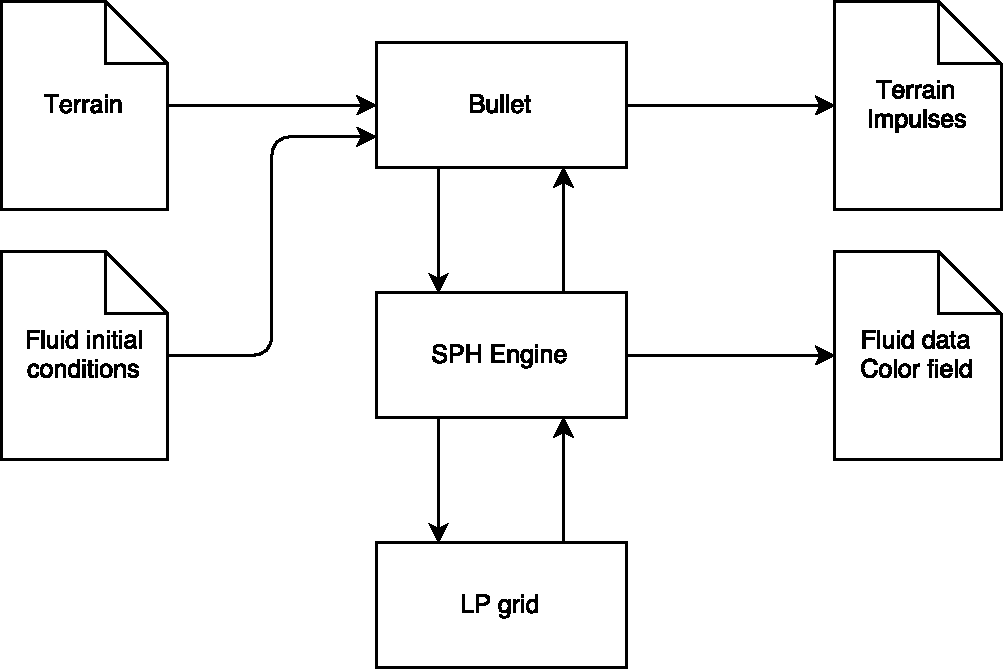
\includegraphics[width=.9\textwidth]{figures/architecture.pdf}
  \caption[Γενική αρχιτεκτονική υλοποίησης] {Διαγραμματική απεικόνιση της γενική
    αρχιτεκτονικής της εφαρμογής προσομοίωσης που υλοποιήθηκε. Το τρισδιάστατο μοντέλο της
    ακτογραμμής και οι αρχικές συνθήκες του ρευστού εισάγονται στη μηχανή φυσικής
    \eng{Bullet}, η οποία σε συνεργασία με την μηχανή \eng{SPH} που αναπτύχθηκε
    αναλαμβάνει την προσομοίωση. Η μηχανή \eng{SPH} χρησιμοποιεί την ειδική δομή δεδομένων
    \eng{LP grid} για την βελτιστοποίηση της πρόσβασης στα σωματίδια της προσομοίωσης. Η
    καταγραφή των ώσεων επάνω στην ακτογραμμή πραγματοποιείται από την \eng{Bullet}, ενώ
    τα δεδομένα του ρευστού εξάγονται από την μηχανή \eng{SPH}.}
  \label{fig:architecture}
\end{figure}
παραγράφους. Μετά από κάθε εσωτερικό βήμα της \eng{Bullet}, η μηχανή \eng{SPH} αναλαμβάνει
τον υπολογισμό δυνάμεων όπως αυτές προκύπτουν από τη μέθοδο \eng{SPH} βάσει της δυναμικής
κατάστασης του ρευστού. Οι δυνάμεις αυτές επανατροφοδοτούνται και πάλι πίσω στην
\eng{Bullet} προκειμένου να ολοκληρωθούν στην κίνηση των σωματιδίων στο επόμενο βήμα της
προσομοίωσης. Όπως είναι φανερό, για την εκτέλεση των υπολογισμών της \eng{SPH} με
αλγόριθμο λογικής υπολογιστικής πολυπλοκότητας, είναι αναγκαίος ο σχεδιασμός ειδικών δομών
δεδομένων, όπως ήδη αναφέρθηκε και στην παράγραφο
\ref{sssec:implementation-techniques}. Για το σκοπό αυτό στην παρούσα εργασία αναπτύχθηκε
το \eng{LP grid}, μια εξειδικευμένη δομή δεδομένων, υπεύθυνη για την αποθήκευση των
σωματιδίων στη μνήμη με τρόπο τέτοιο ώστε να βελτιστοποιείται η πρόσβαση σε αυτά από τη
μηχανή \eng{SPH}. Επιγραμματικά, η δομή αυτή ακολουθεί τη λογική \eng{CLL} με \eng{dynamic
  sliding vector} (εικόνα \ref{fig:particle-storage} επάνω) για την αποθήκευση των
σωματιδίων. Ακολουθείται λογική χωρικής διαμέρισης και διευθυνσιοδότησης (\eng{spatial
  hashing}), καθώς ο χώρος της προσομοίωσης διαιρείται σε κυβικό πλέγμα, όπου το μέγεθος
του κελιού ταυτίζεται με την ακτίνα αλληλεπίδρασης (εξομάλυνσης) των σωματιδίων. Ο σκοπός
της διαμέρισης αυτής είναι η γρήγορη ταυτοποίηση γειτονικών σωματιδίων, τα οποία
ευρισκόμενα σε απόσταση μικρότερης της ακτίνας εξομάλυνσης, συνεισφέρουν στην εκτίμηση
ποσοτήτων μέσω σταθμισμένων αθροισμάτων κατά \eng{SPH}. Τα σωματίδια κάθε κελιού
αποθηκεύονται συνεχόμενα, ενώ τα κελιά αντιπροσωπεύονται με διάταξη κατάλληλη για την κατά
το δυνατόν διατήρηση της τοπικότητας μεταξύ τους, προκειμένου η πρόσβαση σε γειτονικά
κελιά να εκμεταλλεύεται αποδοτικότερα την κρυφή μνήμη. Ένα αξιοσημείωτο επιπρόσθετο
πλεονέκτημα αυτής της οργάνωσης, είναι η δυνατότητα παράλληλης σάρωσης του πλέγματος για
την ανίχνευση αλληλεπιδράσεων μεταξύ σωματιδίων, η οποία αυξάνει σημαντικά την απόδοση της
εφαρμογής.

\paragraph{} Τα δεδομένα που προκύπτουν από την προσομοίωση εξάγονται σε αρχεία κειμένου,
στη μορφή \eng{VTK}, προκειμένου να μπορούν να οπτικοποιηθούν με ποικίλους τρόπους και
συνδυασμούς, εύκολα και διαδραστικά με τη βοήθεια ειδικών για το σκοπό αυτό
προγράμματων. Από τα στοιχεία καταγραφών της \eng{Bullet}, εξάγονται οι δυνάμεις που
δέχθηκε η ακτογραμμή από το ρευστό, τόσο στα μεμονωμένα στιγμιότυπα όσο και αθροιστικά στο
τέλος (σε χάρτη επάνω στο μοντέλο της ακτογραμμής -- \eng{embodied heatmap}), ενώ
λεπτομερή στοιχεία που σχετίζονται με την ίδια τη ροή εξάγονται από τη μηχανή
\eng{SPH}. Αυτά περιλαμβάνουν θέση, ταχύτητα, δυνάμεις πίεσης και ιξώδους, στοιχεία της
προσομοίωσης (όπως ο αριθμός γειτονικών σωματιδίων για κάθε σωματίδιο) αλλά και κανονική
δειγματοληψία του χρωματικού πεδίου (\eng{color field}). Αυτό είναι ένα βαθμωτό πεδίο που
αντιπροσωπεύει την αδιάστατη πυκνότητα του ρευστού στο χώρο, κατάλληλες ισοεπιφάνειες του
οποίου χρησιμοποιούνται για την ανακατασκευή της επιφάνειας του ρευστού από τα σωματίδια.

\subsection{\texorpdfstring{Αναπαράσταση ακτογραμμής και προσομοίωση στην \eng{Bullet}}{}}
\label{ssec:bullet}
\paragraph{} Η \eng{Bullet} είναι μια μηχανή φυσικής που προσομοιώνει ανίχνευση και
χειρισμό συγκρούσεων καθώς και δυναμική εύκαμπτων και στερεών σωμάτων. Χρησιμοποιείται
ευρύτατα στην παραγωγή ηλεκτρονικών παιχνιδιών και οπτικών εφέ σε ταινίες, ενώ διατίθεται
ως ελεύθερο λογισμικό ανοιχτού πηγαίου κώδικα, αναπτυσσόμενη συνεχώς και υποστηριζόμενη
από μεγάλη και ενεργή κοινότητα χρηστών.

\paragraph{} Η \eng{Bullet} είναι σχεδιασμένη βάσει αντικειμενοστραφούς αρχιτεκτονικής,
καθώς οτιδήποτε, ακόμη και ο ίδιος ο κόσμος της εξομοίωσης με τις όποιες ιδιότητές του
αναπαρίσταται με αντικείμενα, τα οποία δημιουργούνται, τροποποιούνται και καταστρέφονται
βάσει των αντίστοιχων μεθόδων της κλάσης τους. Ο κόσμος της προσομοίωσης, που ανήκει στην
κλάση \ttt{btDiscreteDynamicsWorld} δημιουργείται με βάση τέσσερα ορίσματα, εκ των οποίων
δύο (\ttt{btCollisionConfiguration} και \ttt{btDispatcher}) σχετίζονται με τους
αλγορίθμους χειρισμού συγκρούσεων και αφήνονται στις προεπιλεγμένες τους κλάσεις. Το τρίτο
όρισμα (\ttt{btBroadphaseInterface}) αφορά την οργάνωση των σωμάτων της προσομοίωσης στη
μνήμη με σκοπό τον εκ των προτέρων αποκλεισμό συγκρούσεων μεταξύ τους για την ελάφρυνση
του υπολογιστικού φόρτου. Στην παρούσα εργασία επιλέγεται η κλάση \ttt{btDbvtBroadphase} η
οποία ταξινομεί δυναμικά τα σώματα της προσομοίωσης σε δομή δένδρου με βάση τα
προσανατολισμένα με τους άξονες συντεταγμένων περιβάλλοντα κουτιά τους (\eng{AABBs}). Το
τελευταίο όρισμα (\ttt{btConstraintSolver}) καθορίζει τον τρόπο χειρισμού των γεωμετρικών
περιορισμών κατά την προσομοίωση. Εδώ επιλέγεται η χρήση του \eng{SIS} (\eng{Sequential
  Impulse Solver}) για την επίλυση πολλαπλών μηχανικών περιορισμών
\cite{catto2005iterative}. Τα σώματα της προσομοίωσης αρχικοποιούνται όπως περιγράφεται
στις παραγράφους παρακάτω και προστίθενται στον κόσμο της προσομοίωσης με τη μέθοδο
\ttt{addRigidBody}.

\paragraph{} Η ακτογραμμή αναπαρίσταται στο πρόγραμμα σαν ένα στατικό δίκτυο τριγώνων με
ιεραρχικούς περιβάλλοντες όγκους (\ttt{btBvhTriangleMesh}) της \eng{Bullet}. Τα δεδομένα
του τρισδιάστατου μοντέλου εισάγονται από ένα αρχείο τύπου \eng{OBJ} στο τριγωνικό δίκτυο
αφού κανονικοποιηθούν σε κλίμακα βάσει ενός παράγοντα κλιμάκωσης (\eng{scaling factor})
και θέση μετακινούμενα στο χώρο προς την αρχή των αξόνων (\eng{docking}). Γύρω από την
ακτογραμμή δημιουργείται και το όριό της (\eng{terrain boundary}) το οποίο ταυτίζεται με
το προσανατολισμένο στους άξονες περιβάλλον κουτί της (\eng{AABB}). Η κανονικοποιημένη
ακτογραμμή και το όριό της εξάγονται και πάλι σε ένα αρχείο τύπου \eng{OBJ}, το οποίο
χρησιμοποιείται σε συνδυασμό με την οπτικοποίηση των υπόλοιπων δεδομένων. Σε κάθε
εσωτερικό βήμα της προσομοίωσης συλλέγονται οι ώσεις που ασκεί το ρευστό στην ακτογραμμή
σε ειδικό διάνυσμα, το οποίο χρησιμοποιείται για να εξαχθούν οι σχετικές πληροφορίες σε
κάθε στιγμιότυπο.

\paragraph{} Η προσομοίωση του κόσμου διεξάγεται σε διακριτά χρονικά βήματα μέσω της
μεθόδου \ttt{stepSimulation}, η οποία δέχεται τρία ορίσματα, έστω \ttt{T}, \ttt{k} και
\ttt{t} αντίστοιχα. Το πρώτο από αυτά καθορίζει το χρονικό διάστημα που θα προσομοιωθεί
συνολικά μέχρι το επόμενο στιγμιότυπο της προσομοίωσης (για συλλογή δεδομένων), το δεύτερο
το μέγιστο αριθμό εσωτερικών βημάτων εντός αυτού και το τρίτο τη χρονική διάρκεια του
εσωτερικού (αδιαίρετου) βήματος της προσομοίωσης (όπως είναι προφανές, θα πρέπει να ισχύει
\ttt{T$\geq$k*t}). Η \eng{Bullet} παρέχει τη δυνατότητα ορισμού μιας \eng{callback}
συνάρτησης, η οποία καλείται μετά από κάθε εσωτερικό βήμα της προσομοίωσης και όπως θα
αναλυθεί παρακάτω, εκτελεί τον κώδικα που υλοποιεί τη μηχανή \eng{SPH} για την προσθήκη
των δυνάμεων ρευστού στα σωματίδια.

\subsection{\texorpdfstring{Μηχανή \eng{SPH}}{}}
\subsubsection{Αρχικοποίηση}
\label{sssec:fluid-init}
\paragraph{} Σύμφωνα με τη μέθοδο \eng{SPH} όπως περιγράφηκε έως τώρα, το ρευστό
διακριτοποιείται σε σωματίδια τα οποία χρησιμοποιούνται σαν σημεία παρεμβολής σε
σταθμισμένα αθροίσματα για την εκτίμηση των ιδιοτήτων του ρευστού στο χώρο. Λόγω των
σημαντικών αποκλίσεων που μπορούν να προκύψουν εξαιτίας της έλλειψης γειτονικών
σωματιδίων, η μέθοδος ενδείκνυται κυρίως για την προσομοίωση συμπιεστών ρευστών (αερίων),
των οποίων η πυκνότητα δεν είναι σταθερή. Σε ασυμπίεστα ρευστά (υγρά) αντίθετα, όπου τα
όρια είναι σαφή, καθίσταται προβληματικός ο υπολογισμός ποσοτητων κοντά σε αυτά λόγω
μικρού αριθμού και ανομοιογενώς κατανεμημένων στο χώρο γειτονικών σωματιδίων. Για το λόγο
αυτό στην παρούσα προσομοίωση υιοθετήθηκε μια διαφορετική προσέγγιση, όπου τα σωματίδια
διαθέτουν υλική υπόσταση στερεών σφαιρών, η οποία μέσω επίλυσης γεωμετρικών περιορισμών σε
κάθε βήμα της προσομοίωσης (\eng{Position-Based Dynamics -- PBD} \cite{Muller2007109})
εξασφαλίζει την ασυμπιεστότητα του ρευστού \cite{macklin2013position}. Οι γεωμετρικοί
περιορισμοί επιλύονται από την \eng{Bullet}, αποκλείοντας τη δημιουργία εκφυλισμένων
περιπτώσεων όσον αφορά τις θέσεις των σωματιδίων, καθώς αυτά εμποδίζονται από το να
πλησιάσουν περισσότερο από την απόσταση που υπαγορεύει η ονομαστική πυκνότητα του
ρευστού. Επιπλέον, με τη μέθοδο αυτή διευκολύνεται ο χειρισμός των οριακών συνθηκών, χωρίς
να απαιτούνται επιπρόσθετες τεχνικές για την αναπλήρωση γειτονικών σωματιδίων. Για την
αρχικοποίηση του ρευστού δίνεται η θέση του στο χώρο, η αρχική ταχύτητα και το επιθυμητό
πλήθος των σωματιδίων στα οποία πρόκειται να διακριτοποιηθεί.

\begin{figure}[]
  \centering
  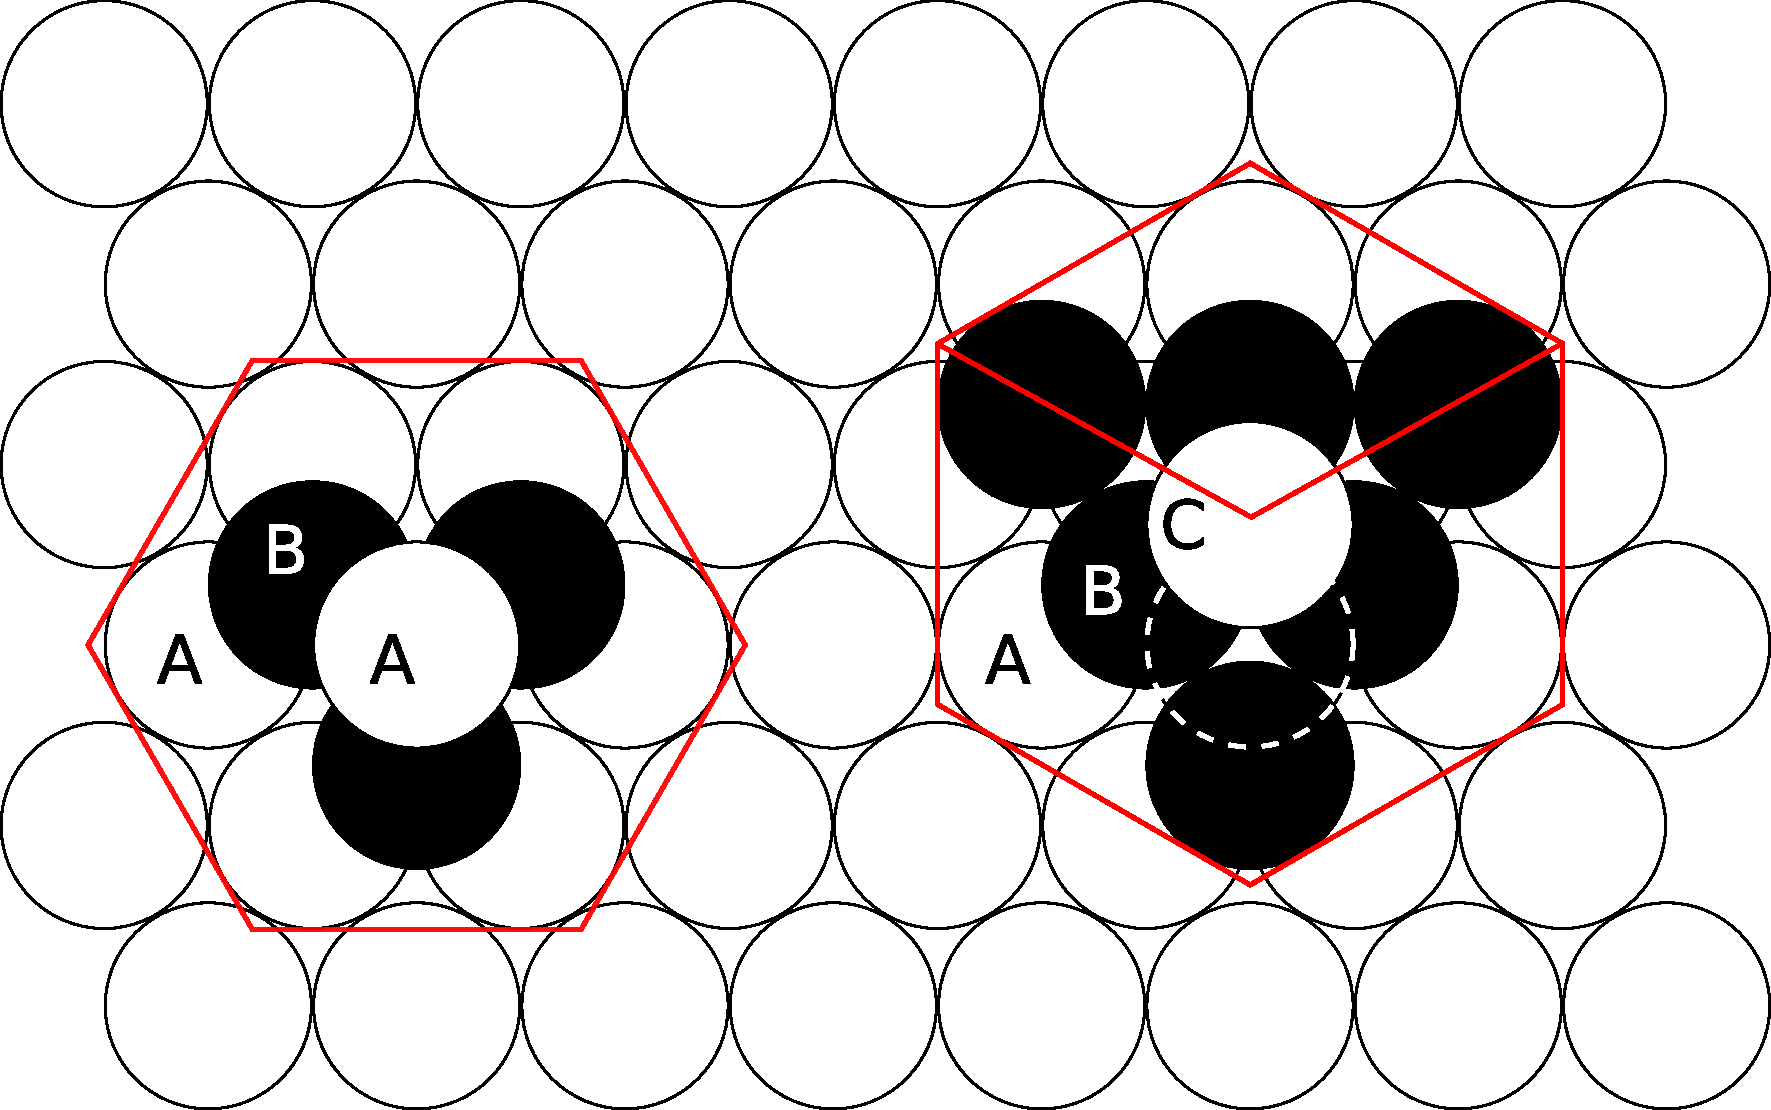
\includegraphics[width=.9\textwidth]{figures/hcp-fcc.pdf}
  \caption[Συνεκτικές διατάξεις σφαιρών] {Σύγκριση συνεκτικών διατάξεων σφαιρών στον
    τρισδιάστατο χώρο, \eng{HCP} αριστερά και \eng{FCC} δεξιά (από
    \ttt{en.wikipedia.org}).}
  \label{fig:hcp-fcc}
\end{figure}

\paragraph{} Για την αρχικοποίηση του ρευστού δίνεται η θέση του στο χώρο, η αρχική
ταχύτητα και το επιθυμητό πλήθος σωματιδίων στα οποία πρόκειται να διακριτοποιηθεί. Τα
σωματίδια προγραμματιστικά είναι δομές \ttt{particle} που εμπλουτίζουν αντικείμενα στερεών
σωμάτων \ttt{btRigidBody} της \eng{Bullet} με πληροφορίες σχετιζόμενες με το ρευστό, όπως
πυκνότητα και πίεση. Η μάζα του ρευστού ισοκατανέμεται στα σωματίδια, τα οποία όντας
σφαιρικού σχήματος τοποθετούνται σε τρισδιάστατο εξαγωνικό πλέγμα \eng{HCP (Hexagonal
  Close-Packed)}, το οποίο επιτυγχάνει τη συνεκτικότερη δυνατή διευθέτηση ίσομεγεθών
σφαιρών με κλάσμα κάλυψης χώρου ίσο με $\pi/(3\sqrt{2})$ (ίδιο με την \eng{FCC}
(\eng{Face-Centered Cubic}), εικόνα \ref{fig:hcp-fcc}). Η διευθέτηση αυτή, η οποία
αποτελεί μία εκ πολλών προτεινόμενων διευθετήσεων \cite{diehl2012generating,
  colagrossi2012particle}, προτιμάται εδώ λόγω της απλότητας και της υψηλής τάξης
συμμετρίας της. Η ακτίνα των σωματιδίων υπολογίζεται από το κλάσμα αυτό και τον όγκο του
ρευστού, ενώ η ακτίνα εξομάλυνσης \ttt{h} τέτοια ώστε κάθε σωματίδιο να διαθέτει περίπου
50 γειτονικά σωματίδια με τα οποία αλληλεπιδρά, αριθμός που προκύπτει εμπειρικά σύμφωνα με
τη βιβλιογραφία. Στη συνέχεια, τα σωματίδια τοποθετούνται στο πλέγμα στις θέσεις
\[
  [x, y, z] = \left[ 2i+[(j+k) \bmod 2], \sqrt{3}[j + \frac{1}{3} (k \bmod 2)],
    \frac{2\sqrt{6}}{3} k \right] r
\]

\paragraph{} Μετά την αρχικοποίηση εξάγονται παράμετροι της προσομοίωσης σχετικά με το
ρευστό:
\begin{description}
\item[Χρονικό βήμα] Το χρονικό βήμα καθορίζεται όπως έχει ήδη αναφερθεί από το κριτήριο
  ευστάθειας \eng{CFL}, με το χαρακτηριστικό μήκος να αποτελεί η ακτίνα των σωματιδίων και
  χαρακτηριστική ταχύτητα τη μέγιστη ταχύτητα των σωματιδίων με βάση την αρχική μηχανική
  ενέργεια του ρευστού.
\item[Πλήθος γειτόνων] Στην αρχική κατάσταση όπου τα σωματίδια είναι διευθετημένα στο
  πλέγμα \eng{HCP}, γίνεται ανίχνευση γειτόνων ώστε να μετρηθεί ο πραγματικός μέγιστος
  αριθμός γειτόνων ένός σωματιδίου (ο οποίος δεν είναι σχεδόν ποτέ ακριβώς 50 λόγω
  διακριτοποίησης).
\item[Καταστατική εξίσωση] Καθώς το πρόβλημα της ασυμπιεστότητας λύνεται άμεσα μέσω της
  επίλυσης γεωμετρικών περιορισμών μεταξύ των σωματιδίων, ως καταστατική εξίσωση
  χρησιμοποιείται η γραμμική των ιδανικών αερίων (σχέση \ref{eq:ideal-state}). Αυτή
  επιτρέπει μεγαλύτερο χρονικό βήμα και ανοχή όσον αφορά την ευστάθεια στις διακυμάνσεις
  της υπολογιζόμενης πυκνότητας. Σε περίπτωση υπολογισμού πολύ χαμηλής πυκνότητας
  μικρότερης από κάποιο κατώφλι (λ.χ. 0.9 της ονομαστικής) αυτή συμβατικά αντικαθίσταται
  από την ονομαστική, θεωρώντας οτι δεν υπάρχουν αρκετα γειτονικά σωματίδια για αξιόπιστη
  εκτίμηση.
\item[Συντελεστής πυκνότητας] Λόγω της εξάρτησης των πυρήνων εξομάλυνσης από την ακτίνα
  εξομάλυνσης, αλλά και της μάζας των σωματιδίων από τη διακριτοποίηση, το σταθμισμένο
  άθροισμα της εκτίμησης της πυκνότητας δεν ισούται με την πραγματική πυκνότητα του
  ρευστού, αλλά σχετίζεται αναλογικά με έναν συντελεστή, ο οποίος εξάγεται κατά το στάδιο
  αυτό. Ο συντελεστής αυτός χρησιμοποιείται για την αναλογική αντιστοίχιση της αδιάστατης
  πυκνότητας με την πραγματική και υπολογίζεται με βάση τη μέγιστη πυκνότητα των
  σωματιδίων κατά την ανίχνευση γειτόνων στην αρχική κατάσταση όπως αναφέρεται παραπάνω.
\end{description}

\subsubsection{Αναπαράσταση}
\label{sssec:lp-grid-representation}
\paragraph{} Στις προσομοιώσεις \eng{SPH} χρησιμοποιούνται διάφορες δομές δεδομένων με
σκοπό τη βελτιστοποίηση της πρόσβασης και ενημέρωσης σε γειτονικά σωματίδια, όπως
αναφέρθηκε και στην παράγραφο \ref{sssec:implementation-techniques}. Για την καλύτερη
απόδοση της παρούσας προσομοίωσης αναπτύχθηκε εξειδικευμένη δομή δεδομένων, στο εξής
καλούμενη \eng{LP grid}, υπεύθυνη όχι μόνο για την αποθήκευση των σωματιδίων, αλλά και
τιμών βαθμωτών πεδίων του χώρου σε ενιαίο πλαίσιο οργάνωσης. Ο χώρος της προσομοίωσης
διαιρείται σε ένα κυβικό πλέγμα προσανατολισμένο με το τρισορθογώνιο σύστημα
συντεταγμένων, με το βήμα του πλέγματος (μήκος πλευράς των κύβων) να ισούται με την ακτίνα
εξομάλυνσης της προσομοίωσης. Με τον τρόπο αυτό όλοι οι γείτονες ενός σωματιδίου
βρίσκονται στα 26 κελιά που περιβάλλουν το κελι στο οποίο ανήκει. Η διάταξη των κελιών στη
μνήμη έχει στόχο την διατήρηση της τοπικότητας (\eng{locality preserving}, εξ ου και η
ονομασία), ώστε κελιά που βρίσκονται κοντά στον τρισδιάστατο χώρο να βρίσκονται κοντά και
στη μνήμη (η οποία είναι μονοδιάστατη και γραμμική). Έτσι, με την αντιγραφή ενός τμήματος
κυρίας μνήμης (\eng{RAM}) στην κρυφή μνήμη (\eng{cache}) αυξάνεται η πιθανότητα τα
δεδομένα γειτονικών σωματιδίων να μεταφέρονται συντονισμένα στην κρυφή μνήμη, με
αποτέλεσμα την αύξηση του λόγου \eng{hit}/\eng{miss} και συνακόλουθα της ταχύτητας του
προγράμματος.

\paragraph{Οργάνωση} Στη δομή \ttt{lp\_grid} αποθηκεύονται διάφορες παράμετροι της
προσομοίωσης όπως η αρχή του (\ttt{origin}), το βήμα του (\ttt{step} που ισούται με την
ακτίνα εξομάλυνσης \ttt{smoothing\_radius}), το πλήθος των κελιών κατά μήκος κάθε άξονα
(\ttt{x}, \ttt{y}, \ttt{z}), όπως και το πλήθος κελιών και σωματιδίων (\ttt{cell\_count},
\ttt{particle\_count}). Επίσης, όπως φαίνεται και στο σχήμα \ref{fig:lp-grid}, η δομή
περιλαμβάνει τρία διανύσματα δεικτών:
\begin{description}
\item[\ttt{MAP}] Στο διάνυσμα αυτό αποθηκεύονται δείκτες προς θέσεις εντός του
  \ttt{anchors}. Σκοπός του \ttt{map} είναι η διευθυνσιοδότηση σύμφωνα με τη βέλτιστη για
  τη διατήρηση της τοπικότητας διάταξή των κελιών (αντιστοίχιση τρισδιάστατου χώρου σε
  μονοδιάστατο). Διαθέτει \ttt{cell\_count+1} θέσεις, με το επιπλέον στοιχείο να
  αντιστοιχεί σε ένα εικονικό κελί που περιέχει σωματίδια εκτός ορίων του πλέγματος.
\item[\ttt{ANCHORS}] Κάθε δείκτης του διανύσματος αυτού σηματοδοτεί την αρχή του εκάστοτε
  κελιού (το πρώτο σωματίδιο) στο διάνυσμα \ttt{particles}. Τα κελιά αντιπροσωπεύονται
  διατεταγμένα προς διατήρηση τοπικότητας στο \ttt{anchors} και τα σωματίδια κάθε κελιού
  αποθηκεύονται σε διαδοχικές θέσεις του \ttt{particles}. Συνεπώς για τα στοιχεία του
  διανύσματος αυτού ισχύει \ttt{a[i-1]} $\leq$
  \ttt{a[i]} (στην περίπτωση που \ttt{a[i-1]} = \ttt{a[i]}, το κελί που αντιστοιχεί στο
  \ttt{a[i-1]} δεν περιέχει κανένα σωματίδιο). Το διάνυσμα διαθέτει και αυτό
  \ttt{cell\_count+1} θέσεις.
\item[\ttt{PARTICLES}] Το διάνυσμα αυτό διαθέτει \ttt{particle\_count+1} θέσεις και
  περιέχει τα σωματίδια της προσομοίωσης, ενώ κάθε πραγματικό κελί \ttt{i} στην
  προσομοίωση αντιπροσωπεύεται από το ζεύγος δεικτών \ttt{a[i]}, \ttt{a[i+1]}. Η επιπλέον
  θέση στο τέλος του διανύσματος χρησιμοποιείται για έγκυρο δείκτη τέλους του τελευταίου
  (εικονικού) κελιού (τα σωματίδια του οποίου αποθηκεύονται στις τελευταίες θέσεις του
  \ttt{particles}), καθώς και για έγκυρη αρχικοποίηση (κατά τη διάρκεια της οποίας, όπως
  θα φανεί παρακάτω, υπάρχει δείκτης προς τη θέση αυτή).
\end{description}
\begin{figure}[h]
  \centering
  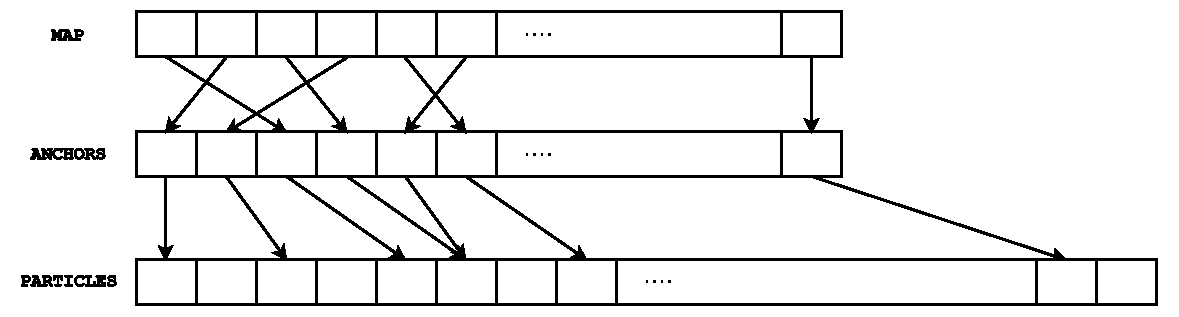
\includegraphics[width=\textwidth]{figures/lp-grid.pdf}
  \caption[Διανύσματα οργάνωσης του \ttt{lp\_grid}] {Τα τρία διανύσματα διευθυνσιοδότησης
    και αποθήκευσης του \ttt{lp\_grid}, μέσω των οποίων επιτυγχάνεται γρήγορη πρόσβαση και
    αποτελεσματική για τη διατήρηση της τοπικότητας διάταξη των σωματιδίων στη μνήμη.}
  \label{fig:lp-grid}
\end{figure}

\paragraph{} Η πρόσβαση στα κελιά του πλέγματος γίνεται με καθοδήγηση μέσω δεικτών
(\eng{pointer cascading}). Έστω οτι ζητούνται τα περιεχόμενα του κελιού στη διεύθυνση
\ttt{(i, j, k)} του πλέγματος. Η τρισδιάστατη διεύθυνση μετατρέπεται σε μονοδιάστατη (έναν
αριθμητικό δείκτη) μέσω μιας συνάρτησης \ttt{linearize}, η οποία αρκεί να υπολογίζει
διαφορετικό αποτέλεσμα για κάθε έγκυρη τρισδιάστατη διεύθυνση εισόδου και να έχει πεδίο
τιμών εντός του διαστήματος \ttt{[0, cell\_count]}, προκειμένου η έξοδος να αποτελεί
έγκυρη διεύθυνση για το διάνυσμα \ttt{map}. Τότε η αρχή του κελίου είναι ο δείκτης
\ttt{a[c] = *map[linearize(i, j, k)]} και το τέλος \ttt{a[c+1]}, με αποτέλεσμα τα
σωματίδια του κελιού να βρίσκονται με έναν απλό βρόχο επανάληψης ανάμεσα στους δύο
δείκτες, συμπεριλαμβανομένου του αρχικού, αλλά όχι του τελικού (δείκτης στο πρώτο
σωματίδιο του επόμενου κελιού).

\begin{figure}[]
  \begin{subfigure}{.5\textwidth}
    \centering
    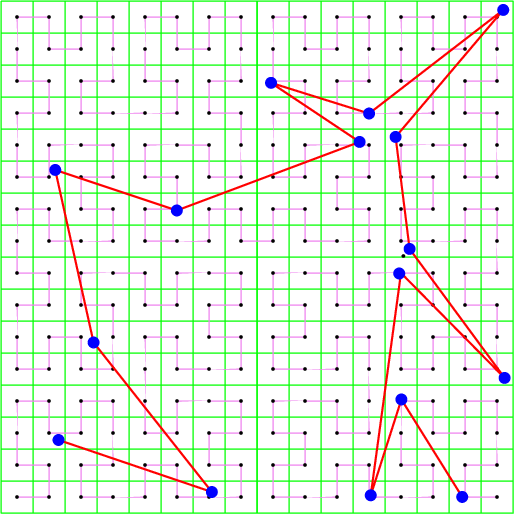
\includegraphics[width=.8\textwidth]{figures/hilbert-sort-middle.png}
  \end{subfigure}
  \begin{subfigure}{.5\textwidth}
    \centering
    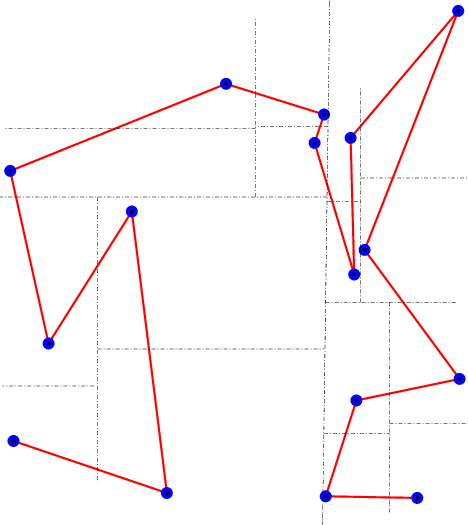
\includegraphics[width=.8\textwidth]{figures/hilbert-sort-median.png}
  \end{subfigure}
  \caption[Χωρική ταξινόμηση]{Δύο διαφορετικοί τρόποι χωρικής ταξινόμησης (\eng{spatial
      sort}) κατά μήκος της καμπύλης \eng{Hilbert}. Αριστερά διαχωρίζοντας κάθε
    υποτετράγωνο στο μέσο, δεξιά κατασκευάζοντας ένα δισδιάστατο δένδρο προσαρμοσμένο στο
    σύνολο σημείων, εναλλακτικά για τους δύο άξονες επιλέγοντας σαν οδηγό το μεσαίο
    (\eng{median}) σημείο (εικόνα από \ttt{doc.cgal.org})}
  \label{fig:spatial-sort}
\end{figure}

\paragraph{Αρχικοποίηση} Η δημιουργία του \ttt{lp\_grid} γίνεται σε τέσσερα στάδια:
\begin{enumerate}
\item Καθορίζεται η αρχή του πλέγματος, το βήμα, το πλήθος κελιών και σωματιδίων του και
  δεσμεύεται βάσει αυτών χώρος στη μνήμη.

\item Τα κελιά του πλέγματος ταξινομούνται στο χώρο (\eng{spatial sort}, εικόνα
  \ref{fig:spatial-sort}) κατά μήκος μιας καμπύλης πλήρωσης χώρου (\eng{space-filling
    curve}, όπως η διάταξη \eng{Z} και η καμπύλη \eng{Hilbert}), με στόχο τη διατήρηση της
  τοπικότητας στην τελική γραμμική διάταξη κατά το μέγιστο δυνατό βαθμό. Στη συνέχεια
  αρχικοποιείται το διάνυσμα \ttt{map}, ώστε στη θέση \ttt{map[linearize(i, j, k)]} να
  υπάρχει δείκτης στην αντίστοιχη θέση του \ttt{anchors} σύμφωνα με τη χωρική ταξινόμηση
  των κελιών.

\item Κατασκευάζεται το διάνυσμα \ttt{cell\_pc} στις θέσεις του οποίου αποθηκεύεται το
  πλήθος των σωματιδίων σε κάθε κελί. Κατά τη διαδικασία αυτή χρησιμοποιείται η συνάρτηση
  \ttt{particle\_anchor}, η οποία παίρ\-νει ως όρισμα το \ttt{lp\_grid} και ένα σωματίδιο
  και επιστρέφει ένα δείκτη στον \ttt{anchor} του κελιού που περιέχει το σωματίδιο. Στη
  συνέχεια σύμφωνα με το \ttt{cell\_pc} αρχικοποιούνται οι δείκτες στο διάνυσμα
  \ttt{anchors}.

\item Τα σωματίδια αποθηκεύονται στο διάνυσμα \ttt{particles}, στη θέση που δείχνει ο
  \ttt{anchor} του κελιού που ανήκουν, ενώ μετά από κάθε προσθήκη ο \ttt{anchor} αυξάνεται
  κατά 1 (δείχνει στην επόμενη θέση του \ttt{particles}). Στο τέλος της διαδικασίας κάθε
  \ttt{anchor} δείχνει στην αρχή του επόμενου κελιού (και ο τελευταίος στην τελευταία
  επιπλέον θέση του \ttt{particles}). Ο πρώτος \ttt{anchor} επαναφέρεται στην αρχή του
  \ttt{particles} και κάθε επόμενος εκεί που δείχνει ο προηγούμενός του.
\end{enumerate}
Ακολουθεί ψευδοκώδικας για τη συνάρτηση \ttt{make\_lp\_grid} που δημιουργεί ένα
\ttt{lp\_grid}\footnote{Ονόματα μεταβλητών που λήγουν σε \ttt{p} υποδηλώνουν οτι η
  μεταβλητή αποτελεί δείκτη}: \selectlanguage{english}
\begin{verbatim}
lp_grid make_lp_grid(domain dom, fluid fl)
|   lp_grid lpg;
|   allocate_lp_grid (&lpg, dom, fl);
|   point cc[lpg.cell_count] = spatial_sort(collect_cell_centers(lpg));
|
|   // MAP initialization according to spatial sort.
|   for int i = 0 below lpg.cell_count:
|   |   lpg.map[linearize(cc[i].x, cc[i].y, cc[i].z)] = lpg.anchors + i;
|   lpg.map[lpg.cell_count] = lpg.anchors + lpg.cell_count;
|
|   // Store the particle count for each cell.
|   ptrdiff cell_pc[lpg.cell_count+1] = {0};
|   for particle p in fl.particles:
|   |   cell_pc[particle_anchor(lpg, p) - lpg.anchors]++;
|   for int anchor_offset = 0; int i = 0 upto lpg.cell_count:
|   |   lpg.anchors[i] = lpg.particles + anchor_offset;
|   |   anchor_offset += cell_pc[i];
|
|   // Populate particle array and reset anchors
|   for particle p in fl.particles:
|   |   anchor* ap = particle_anchor(lpg, p);
|   |   **ap = p;
|   |   (*ap)++;
|   for int i = lpg.cell_count above 0:
|   |   lpg.anchors[ai] = lpg.anchors[ai-1];
|   lpg.anchors[0] = lpg.particles;
|
|   return lpg;
\end{verbatim}
\selectlanguage{greek}

\paragraph{Ενημέρωση} Μετά από κάθε βήμα της προσομοίωσης τα σωματίδια έχοντας μετακινηθεί
ενδέχεται να βρίσκονται σε διαφορετικό κελί του πλέγματος, το οποίο πρέπει πλέον να
ενημερωθεί. Τα σωματίδια ελέγχονται με τη σειρά και σε περίπτωση σφάλματος, γίνεται
κυκλική μετακίνηση κατά μία θέση (\eng{shift}) δεξιά/αριστερά στο τμήμα του διανύσματος
\ttt{particles} μεταξύ της τρέχουσας και ορθής θέσης του σωματιδίου και αντίστοιχη
μετακίνηση ($\pm 1$) των \ttt{anchors} του τμήματος αυτού. Στη χειρότερη περίπτωση η
διαδικασία αυτή έχει απαγορευτική ασυμπτωτική συμπεριφορά ($Ο(n^2)$) σε συνήθεις όμως
περιπτώσεις απαιτεί πολύ λιγότερο χρόνο, διότι:
\begin{itemize}
\item Κατά κανόνα μικρό πλήθος σωματιδίων αλλάζουν κελί σε κάθε βήμα, δεδομένου οτι τα
  κελιά είναι αρκετά μεγάλα σε σχέση με το μέγεθος και την ταχύτητα των σωματιδίων.
  
\item Η διατήρηση της τοπικότητας εξασφαλίζει οτι τα κελιά άφιξης και προορισμού του
  σωματιδίου (τα οποία αναμένεται να είναι γειτονικά σε λογικό χρονικό βήμα) βρίσκονται
  κοντά στη γραμμική αναπαράσταση, με αποτέλεσμα η διαδικασία ενημέρωσης να αφορά μικρό
  τμήμα των διανυσμάτων \ttt{particles} και \ttt{anchors}.
\end{itemize}

\paragraph{} Στη συνέχεια παρατίθεται ψευδοκώδικας για τη συνάρτηση
\ttt{update\_lp\_grid}\footnote{Μεταβλητές των οποίων το όνομα ξεκινά με \ttt{i} αφορούν
  την τρέχουσα/αρχική θέση του σωματιδίου (\eng{initial}) πριν την ενημέρωση, ενώ με
  \ttt{t} την τελική/ορθή (\eng{terminal})}: \selectlanguage{english}
\begin{verbatim}
void update_lp_grid (lp_grid lpg)
|   anchor ta;
|   particle tmp_storage;
|   for anchor* iap = lpg.anchors below lpg.anchors + lpg.cell_count:
|   |   for anchor ia = *iap below *(iap + 1):
|   |   |   anchor* tap = particle_anchor(lpg, *ia);
|   |   |   if iap != tap:
|   |   |   |   tmp_storage = *ia;
|   |   |   |   if iap < tap:
|   |   |   |   |   ta = *tap - 1;
|   |   |   |   |   for anchor* ap = iap + 1 upto tap: (*ap)--;
|   |   |   |   |   for anchor a = ia below ta: *a = *(a + 1);
|   |   |   |   |   *ta = tmp_storage;
|   |   |   |   |   ia--;
|   |   |   |   else:
|   |   |   |   |   ta = *(tap + 1);
|   |   |   |   |   for anchor* ap = iap above tap: (*ap)++;
|   |   |   |   |   for anchor a = ia above ta: *a = *(a - 1);
|   |   |   |   |   *ta = tmp_storage;
|   return;
\end{verbatim}
\selectlanguage{greek}

\paragraph{} Όπως φαίνεται παραπάνω, στο βρόχο επανάληψης ελέγχεται κάθε σωματίδιο για το
αν βρίσκεται αποθηκευμένο στο τμήμα του \ttt{particles} που αντιστοιχεί στο κελί στο οποίο
βρίσκεται βάσει της θέσης του στο χώρο. Αν βρίσκεται αριστερότερα, μετακινείται στην πρώτη
θέση του ορθού κελιού αποθήκευσης μέσω αριστερής κυκλικής ολίσθησης ανάμεσα στις δύο
θέσεις, ενώ στην αντίθετη περίπτωση μετακινείται στην τελευταία του θέση μέσω δεξιάς
κυκλικής ολίσθησης μεταξύ αυτών των θέσεων. Στη συνέχεια ενημερώνονται κατάλληλα οι
\ttt{anchors} που δείχνουν στο τμήμα όπου λαμβάνει χώρα η ολίσθηση. Τέλος, στην περίπτωση
αριστερής ολίσθησης στην τρέχουσα θέση του βρόχου ελέγχου βρίσκεται μη ελεγμένο σωματίδιο
και για το λόγο αυτό η μεταβλητή ελέγχου του βρόχου \ttt{ia} μειώνεται κατά ένα (ο έλεγχος
γίνεται από τα αριστερά προς τα δεξιά στο διάνυσμα \ttt{particles}).

\subsubsection{Προσομοίωση}
\label{sssec:simulation}
\paragraph{} Για τον υπολογισμό των ιδιοτήτων του ρευστού είναι απαραίτητος ο υπολογισμός
πολλών σταθμισμένων αθροισμάτων που εξαρτώνται απο τις ιδιότητες αλλά και την απόσταση
μεταξύ σωματιδίων. Για να εξασφαλιστεί η διατήρηση της ορμής, οι αμοιβαίες συνεισφορές στα
αθροίσματα αυτά συμμετρικοποιούνται (\ref{sssec:vector-calc}), με αποτέλεσμα να λαμβάνουν
τη μορφή αλληλεπίδρασης. Συνεπώς ο υπολογιστικός φόρτος μειώνεται στο μισό εάν κάθε
αλληλεπίδραση ληφθεί υποψη μία φορά για κάθε ζεύγος σωματιδίων, εξετάζοντας μόνο τα μισά
κελιά γύρω από το τρεχον κελί κατά τη σάρωση του πλέγματος (αυτά που έχουν ελεγχθεί
νωρίτερα, προκειμένουν να αυξηθεί η πιθανότητα τα σωματίδιά τους να βρίσκονται ήδη στην
κρυφή μνήμη). H σάρωση του πλέγματος εκτελείται παράλληλα από πολλά νήματα
(\eng{threads}), μετά το διαχωρισμό του πλέγματος σε τμήματα (\eng{segments}) καταλλήλου
μεγέθους, το οποίο καθορίζεται κατά την αρχικοποίηση του \eng{LP grid}. Εμπειρικά
υιοθετήθηκε ως μέγεθος τμήματος σε κάθε διάσταση η τετραγωνική ρίζα του μήκους της, καθώς
επιτυγχάνει ικανοποιητικό συμβιβασμό μεταξύ κατανομής υπολογιστικού φόρτου (\eng{load
  distribution}) και επιπρόσθετου έργου (\eng{overhead}).

\paragraph{} Η προσομοίωση πραγματοποιείται σε σταθερό εσωτερικό χρονικό βήμα και ανά
συγκεκριμένο αριθμό βημάτων εξάγεται και ένα στιγμιότυπο (\eng{frame}), το οποίο περιέχει
πληροφορίες για τα σωματίδια, το ρευστό και την ακτογραμμή. Τα αρχεία \eng{VTK} που
αναπαριστούν το στιγμιότυπο ονομάζονται σύμφωνα με τον αύξοντα αριθμό αυτού, ώστε τελικά
να σχηματίζουν μια χρονοσειρά (\eng{file-} ή \eng{time-series}). Οι συγκρούσεις και οι
περιορισμοί ανάμεσα στα υλικά σώματα επιλύονται από την \eng{Bullet}, ενώ οι εσωτερικές
δυνάμεις του ρευστού υπολογίζονται μέσω κατάλληλα ορισμένης συνάρτησης που καλείται μετά
από κάθε εσωτερικό βήμα στον κύριο βρόχο της προσομοίωσης (\eng{tick callback}). Συνοπτικά
εντός αυτής εκτελούνται τα εξής βήματα:

\begin{enumerate}
\item Καταγραφή/αποθήκευση των ώσεων (\eng{impulses}) του ρευστού προς την ακτογραμμή.

\item Ενημέρωση του πλέγματος αποθήκευσης των σωματιδίων.

\item Καθαρισμός δεδομένων των σωματιδίων που πρόκειται να επανυπολογιστούν.

\item Ανιχνευση αλληλεπιδράσεων με σάρωση όλου του πλέγματος.

\item Υπολογισμός πυκνότητας στις θέσεις των σωματιδίων μέσω προοδευτικής άθροισης των
  αμοιβαίων συνεισφορών των αλληλεπιδρώντων ζευγών.

\item Υπολογισμός πίεσης στις ίδιες θέσεις μέσω της καταστατικής εξίσωσης του ρευστού,
  συναρτήσει της πυκνότητας.

\item Υπολογισμός και εφαρμογή των ώσεων που υπολογίζονται ως το γινόμενο των δυνάμεων
  πίεσης/ιξώδους και του χρονικού βήματος. Οι δυνάμεις είναι αντισυμμετρικές σε κάθε
  ζεύγος αλληλεπίδρασης, και οι μεν πίεσης είναι ανάλογες της διαφοράς πίεσης μεταξύ των
  δύο σημείων, οι δε ιξώδους της διαφοράς ταχυτήτων.
\end{enumerate}

\paragraph{} Για την ανακατασκευή της επιφάνειας του ρευστού υπολογίζεται σε διατεταγμένα
σημεία το χρωματικό πεδίο (\eng{color field}), ένα βαθμωτό πεδίο που ισοδυναμεί με την
αδιάστατη πυκνότητα του ρευστού σε κάθε σημείο του χώρου (δηλαδή υπό την παραδοχή οτι κάθε
σωματίδιο έχει μάζα ίση με 1). Τα κελιά του πλέγματος υποδιαιρούνται σε κυβικά υποκελιά,
στις γωνίες των οποίων υπολογίζονται οι τιμές του χρωματικού πεδίου, από τις οποίες στη
συνέχεια οπτικοποιείται η επιφάνεια του ρευστού ως ισοεπιφάνεια του πεδίου. Παρόμοια, για
τη συνολική απεικόνιση των ώσεων του ρευστού προς την ακτογραμμή, κατασκευάζεται το
αθροιστικό πεδίο ώσεων (\eng{impulse field}). Τα δείγματα του πεδίου αυτού υπολογίζονται
στα ίδια σημεία με το χρωματικό πεδίο προσθέτοντας το μέτρο κάθε καταγραφόμενης ώσης στο
κοντινότερο σημείο δειγματοληψίας μετά από κάθε βήμα της προσομοίωσης.

%%% Local Variables:
%%% mode: latex
%%% TeX-master: "report"
%%% End:
